\section {An Introduction to Banana}

Banana (\textit{Musa} spp.) is frequently reported as one of the world’s top agricultural commodities. Annual global production of bananas (including plantain) steadily increased from 98.4 million tonnes in 2000 to an estimated 155.2 million tonnes in 2018 (\ac{FAO}, 2020). A staple food and cash crop of significant agricultural, financial, and social importance, only around 15\% of bananas produced worldwide are traded in international markets, the remaining 85\% are consumed locally (\ac{FAO}, 2018), highlighting the value of bananas as a subsistence crop. Particularly in developing countries where fruits can account for 25\% of daily calorie intake and act as a source of income (\ac{FAO}, 2018).

\subsection{Anatomy and Classification of Banana}  

Banana is a monocotyledonous, herbaceous perennial which belongs to the Musaceae family in the order Zingiberales (Table ~\ref{tab:TaxonTable}) (Schoch \et 2020). Currently, there are 74 species of \textit{Musa} accepted by the World Checklist of Selected Plant Families (WCSP, 2022), including wild, ornamental, and cultivated species. Linnaeus originally described two species of banana: \textit{M. sapientum }and \textit{M. paradisiaca}. However, the classification of banana using the formalised binomial system following Linnaeus proved ineffective due to banana’s complicated genetic history (Cheesman, 1947).  

% Please add the following required packages to your document preamble:
% \usepackage{longtable}
% Note: It may be necessary to compile the document several times to get a multi-page table to line up properly
\begingroup
\setlength{\tabcolsep}{15pt} % Default value: 6pt
\renewcommand{\arraystretch}{0.9}
\begin{longtable}[c]{cc}
\caption[Taxonomy of \textit{Musa} genus]{\textbf{Taxonomy of \textit{Musa} genus including 3 example species} (Schoch et al., 2020, WCSP, 2022).}
\label{tab:TaxonTable}\\
\hline
\textbf{Kingdom}     & Plantae       
\endfirsthead
%
\multicolumn{2}{c}%
{{\bfseries Table \thetable\ continued from previous page}} \\
\endhead
%
\textbf{Phylum}      & Tracheophytes \\ 
\textbf{Class}       & Magnoliopsida \\ 
\textbf{Super order} & Lilianae      \\ 
\textbf{Order}       & Zingiberales  \\ 
\textbf{Family}      & Musaceae      \\ 
\textbf{Genus}       & \textit{Musa} \\ 
\textbf{Species} & \textit{\begin{tabular}[c]{@{}c@{}}M. acuminata,\\
M. balbisiana, \\
M. basjoo\end{tabular}} \\ \hline
\end{longtable}
\endgroup

In the mid-20th century, Cheesman, (1947) recognised the two species described by Linnaeus to be cultivars of wild the \textit{Musa} species \textit{M. acuminata }and \textit{M. balbisiana} and regrouped the remaining \textit{Musa} species into 4 ‘sections’. Building on the work of Cheesman, Simmonds and Shepherd, (1955) developed a genome-based, informal nomenclature system for cultivated banana which is still used today. The system classifies varieties into genome groups based on the ploidy contribution of their wild ancestors, where the species contribution is denoted by the letters ‘A’ and ‘B’ for \textit{M. acuminata} and \textit{M. balbisiana}, respectively. For example, “Cavendish banana (\textit{Musa }spp. AAA group) cv. ‘Grand Nain’” indicates the variety’s sub-group (Cavendish), genus (\textit{Musa}), genome group scoring (AAA), and cultivar (Grand Nain).

The anatomy of banana plants is outlined in detail by Robinson and Saúco, (2010) and Bakry \et (2009). Briefly, plants produce a fibrous root system from a tuberous rhizome. Extended horizontal growth, typical of most rhizomatous plants, is not observed in banana; the plant instead produces suckers which successively grow outwards from the short rhizome. The leaves are produced from the central meristem of the rhizome, or developing sucker, and laminae continue to widen until they mature. As leaf sheaths develop, they become tightly packed and thicken to form the pseudostem which elongates as more leaves emerge to 1-8m in height (Bakry \et 2009) (Figure ~\ref{fig:Anatomy of fruiting banana plant}). 

\begin{figure}[hp]
    \centering
    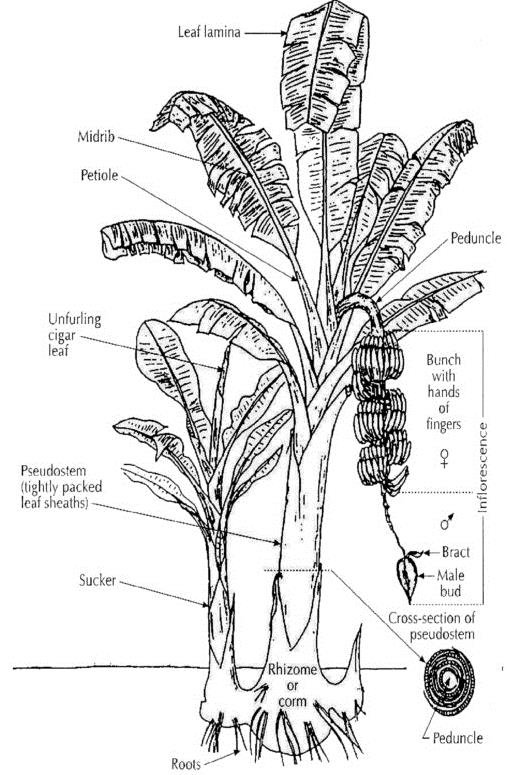
\includegraphics[width=12cm]{Figures/Diagrammatic-representation-of-a-fruiting-banana-plant-with-suckers-in-Bakry-et-al_W640.jpg}
    \caption[Anatomy of fruiting banana plant]{\textbf{Anatomy of fruiting banana plant} (From Bakry, et al. (2009)).}
    \label{fig:Anatomy of fruiting banana plant}
\end{figure}

\subsection{The History, Cultivation, and Value of Banana}

Originating from Southeast Asia, naturally occurring parthenocarpic – development of fruit without fertilisation – individuals of banana have been cultivated for about 10,000 years. Evidence of this can been seen in \textit{Musa banksii} phytoliths discovered in the Kuk swamp in Papua New Guinea (Denham, 2011). Cultivated bananas were spread from Papua New Guinea, hybridising with other subspecies of \textit{M. acuminata} and \textit{M. balbisiana} in the Philippines and northern New Guinea (Perrier \et 2009). Triploid cultivars were produced as a consequence and were dispersed throughout Southeast Asia, Northern Australia, East Africa, and South Asia by the Austronesian peoples; where, although primarily cultivated as a food crop, banana was used in traditional medicine to treat ailments including dysentery, ulcers, leprosy, epilepsy and insect bites (Kumar \et 2012). In these regions, banana has also been used as fodder; in domestic materials, such as plates, children’s toys and dyes; in building for shelter, rafts, or rope; and has significant social and cultural value, involved in many traditional rituals and customs (Hapsari \et 2017).  

Banana cultivation continued to move into the Middle East and Northern Africa from the centre of domestication in Southeast Asia, which can be seen in references banana in Islamic texts such as Ibn al-'Awwam's 12th-century agricultural work, Book on Agriculture (Clément-Mullet, 1866). During expeditions in Southeast Asia and Africa in the mid-1500s, bananas were encountered by Europeans (Amano \et 2021) who transported plants to South America where colonists established banana plantations to supply the USA and Europe (Guzmán-Rivas, 1960, Salas-Pascual and Cáceres-Lorenzo, 2022). This legacy continues today, with over 70\% of the EU’s banana supply coming from South American countries (EuropeanUnion, 2022).  

Banana production takes place year-round in tropical and subtropical regions, where plants are commercially grown as a monoculture crop. Plants are also cultivated by smallholders and in subsistence production systems (Viljoen \et 2020). Commercially, fruits are harvested within about 9-12 months of planting (either\textit{ in vitro} propagated material or suckers) and are grown as a ratoon crop – the plant is cut back to the rhizome once the fruit has been harvested and left to regrow – for several years, by which time yields will have reduced and a new plantation must be generated (BananaLink, 2020). The world’s largest banana growers are India and China which produced over 30 million tonnes and 11 million tonnes in 2018, respectively.  Currently, up to 40\% of all global banana production (domestic and export markets) is reliant on the Cavendish bananas (Warman and Aitken, 2018), a triploid, clonally propagated subgroup deriving from \textit{M. acuminata}. 

\subsection{Bananageddon! \textit{\acl{Fo}} and Current Banana Production}

In recent decades, there have been increasing reports of a potential ‘Bananageddon!’, whereby global banana production is decimated by the soil-borne, fungal pathogen \acl{Focub} (\ac{tr4}), the causative agent of Fusarium wilt of banana (syn. Panama disease). The global banana community’s concern is reflected in the establishment of the \ac{tr4} Task Force as part of the \ac{FAO}'s \ac{wbf}, the Peruvian government’s decision to declare a National Emergency upon the discovery of \ac{Focub} \ac{tr4} in 2021 (FAO, 2021), and in the recent publication by van Westerhoven \et (2022), where the authors stress the threat \ac{Focub} poses to African food security.   

\section{An Introduction to \acl{Focub}}

\subsection{A Brief History of Fusarium Wilt}

The robust response to \ac{Focub4} s not unfounded. During the first half of the 20th century, \ac{Focub} \ac{r1} devastated global production until the resistant banana subgroup, Cavendish, was identified. \ac{Focub} \ac{r1} destroyed approximately 40,000 hectares of ‘Gros Michel’ plantations (Agrios, 2005), and resulted in estimated economic losses of \$400 million (USD) between 1940 and 1960 (Ploetz, 2005). \ac{Focub} \ac{r1} led to the disappearance of ‘Gros Michel’ as an export banana in the 1960s (Molina \et 2007).  

Cavendish bananas were identified as resistant to \ac{Focub} \ac{r1} and subsequently replaced ‘Gros Michel’ (Ordonez \et 2015). However, from the 1960s Cavendish banana plants in Taiwan were observed displaying symptoms of \ac{Focub} infection (Agrios, 2005). Identified in 1994 as \acl{Focub4} (Ploetz, 1994), the strain affecting Cavendish bananas has continued to spread. \ac{Focub4} is now found in Africa, Asia and Europe (Ploetz, 2015a, Thangavelu \et 2019) and is gaining a foothold in South America with recent incursions in Columbia in 2019 (Garcia-Bastidas \et 2019), Peru in 2021 (\ac{FAO}, 2021), and Venuzuela in 2023 (Herrera, \et 2023).

\subsection{Disease Development of \acl{Focub}}

As a soil-borne pathogen, \ac{Focub} first colonises the roots. Asexual spores found in the soil germinate in response to host root exudates. Infection hyphae produced from resting spores (chlamydospores) penetrate the root epidermis at the tip. \ac{Focub} hyphae progress through the root cortex to the rhizome. \ac{Focub} migrates through the xylem in the outer leaf sheaths of the pseudostem occluding vessels and interferes with nutrient uptake and upward water transport; often before external symptoms are observed (Li \et 2017a, Warman and Aitken, 2018). Two asexual spore types, microconidia and macroconidia, are produced within the xylem and help \ac{Focub} overcome some of the host’s barriers, such as naturally occurring end walls or perforation plates of the xylem strands which somewhat inhibit pathogen movement through the host (Dita \et 2018). Xylem vessels begin to collapse, and external symptoms are observed. Tissues become chlorotic and the plant withers as it transpires more than it can translocate. Once the plant dies, the fungus begins to invade other plant tissues and sporulate, particularly on the plant surface, producing chlamydospores (Figure ~\ref{fig:MyLifeCylce}). Chlamydospores can persist in the soil for decades and are resistant to adverse conditions (Pegg \et 2019).  

\begin{figure}[hp!]
    \centering
    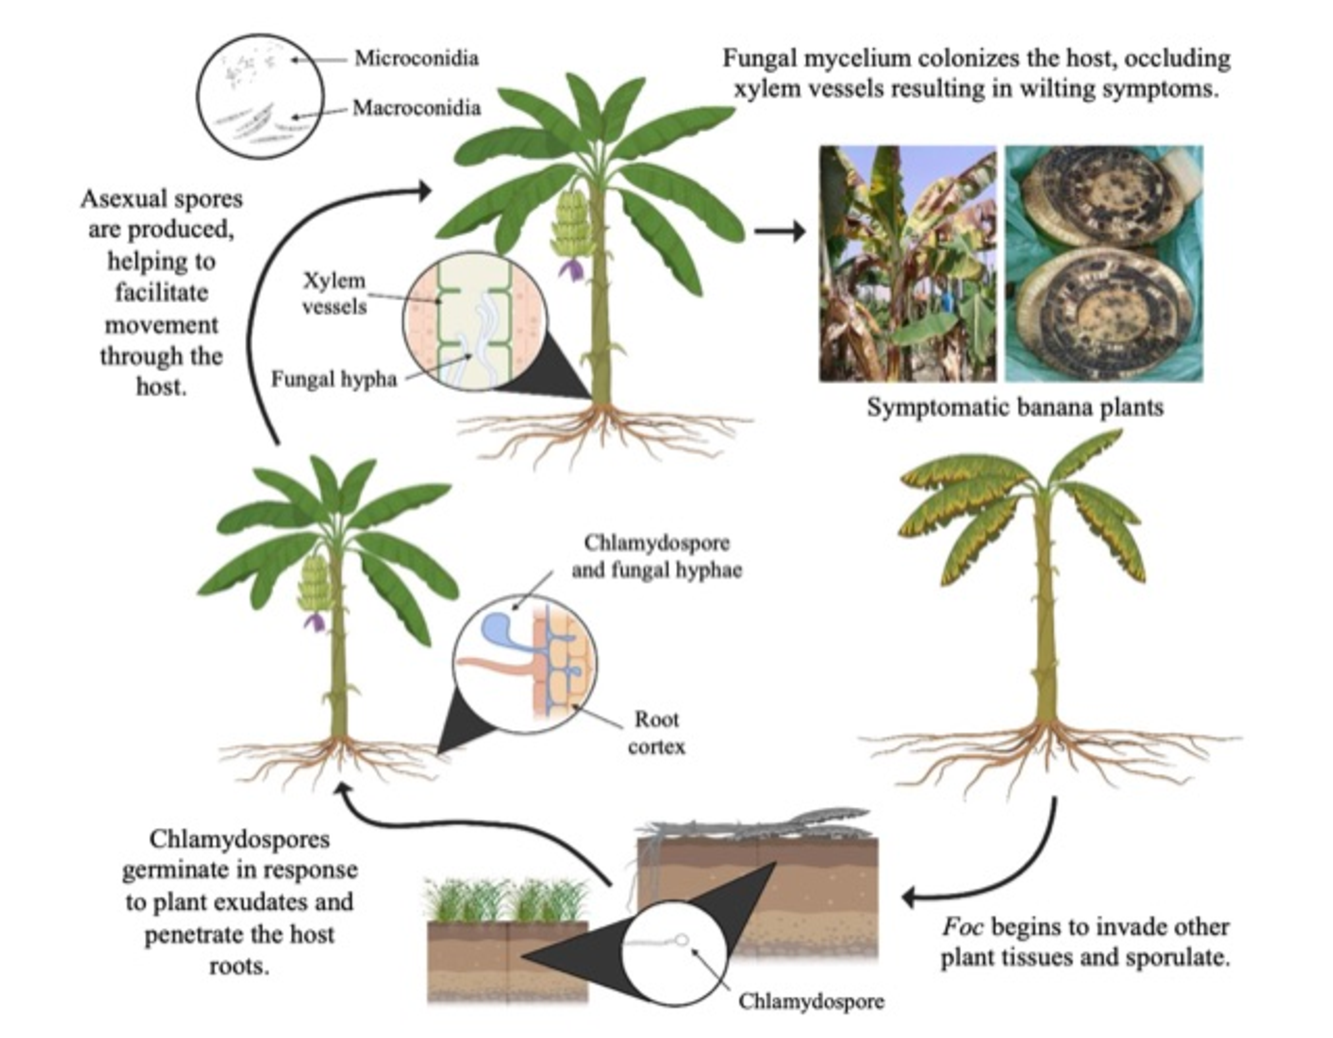
\includegraphics[width=14cm]{Figures/MyLifeCylceNarrow.pdf}
    \caption[Fusarium wilt of banana disease cycle.]{\textbf{Fusarium wilt of banana disease cycle.} Chlamydospores germinate in the soil in response to plant root exudates. Infection hyphae from Chlamydospores penetrate the root tip epidermal cells and progress through then host root cortex to the xylem. Microconidia and macroconidia are produced in the xylem and help to facilitate pathogen movement through the host. As Foc migrates through the xylem it occludes vessels and interferes with nutrient uptake and upward water transport. External wilting symptoms begin to develop; tissues become chlorotic and the plant withers as it transpires more than it can translocate. Eventually, the plant dies, and asexual spores are formed on the dead tissue. Chlamydospores persist in the soil or Foc survives endophytically in an alternative host species. Fungal hyphae are shown in blue. Images of Foc spores adapted from Fourie \et  (2011) and symptomatic banana plant images sourced from Maymon \et  (2020). Figure created with BioRender.com.}
    \label{fig:MyLifeCylce.}
\end{figure}


Alternative hosts, including many grass and weed species, also act as a reservoir of inoculum (Hennessy \et 2005).  \ac{Focub} is dispersed through the movement of contaminated plant and soil material, water, wind, and people. Typical symptoms of \ac{Focub} infection include pseudostem splitting and discolouration, yellowing of lower leaves often forming a ‘skirt’ around the plant, and, occasionally, a streaking pattern is observed on the foliage (Figure ~\ref{fig:FusariumWiltSymptoms}). 

\begin{figure}[hpt!]
    \centering
    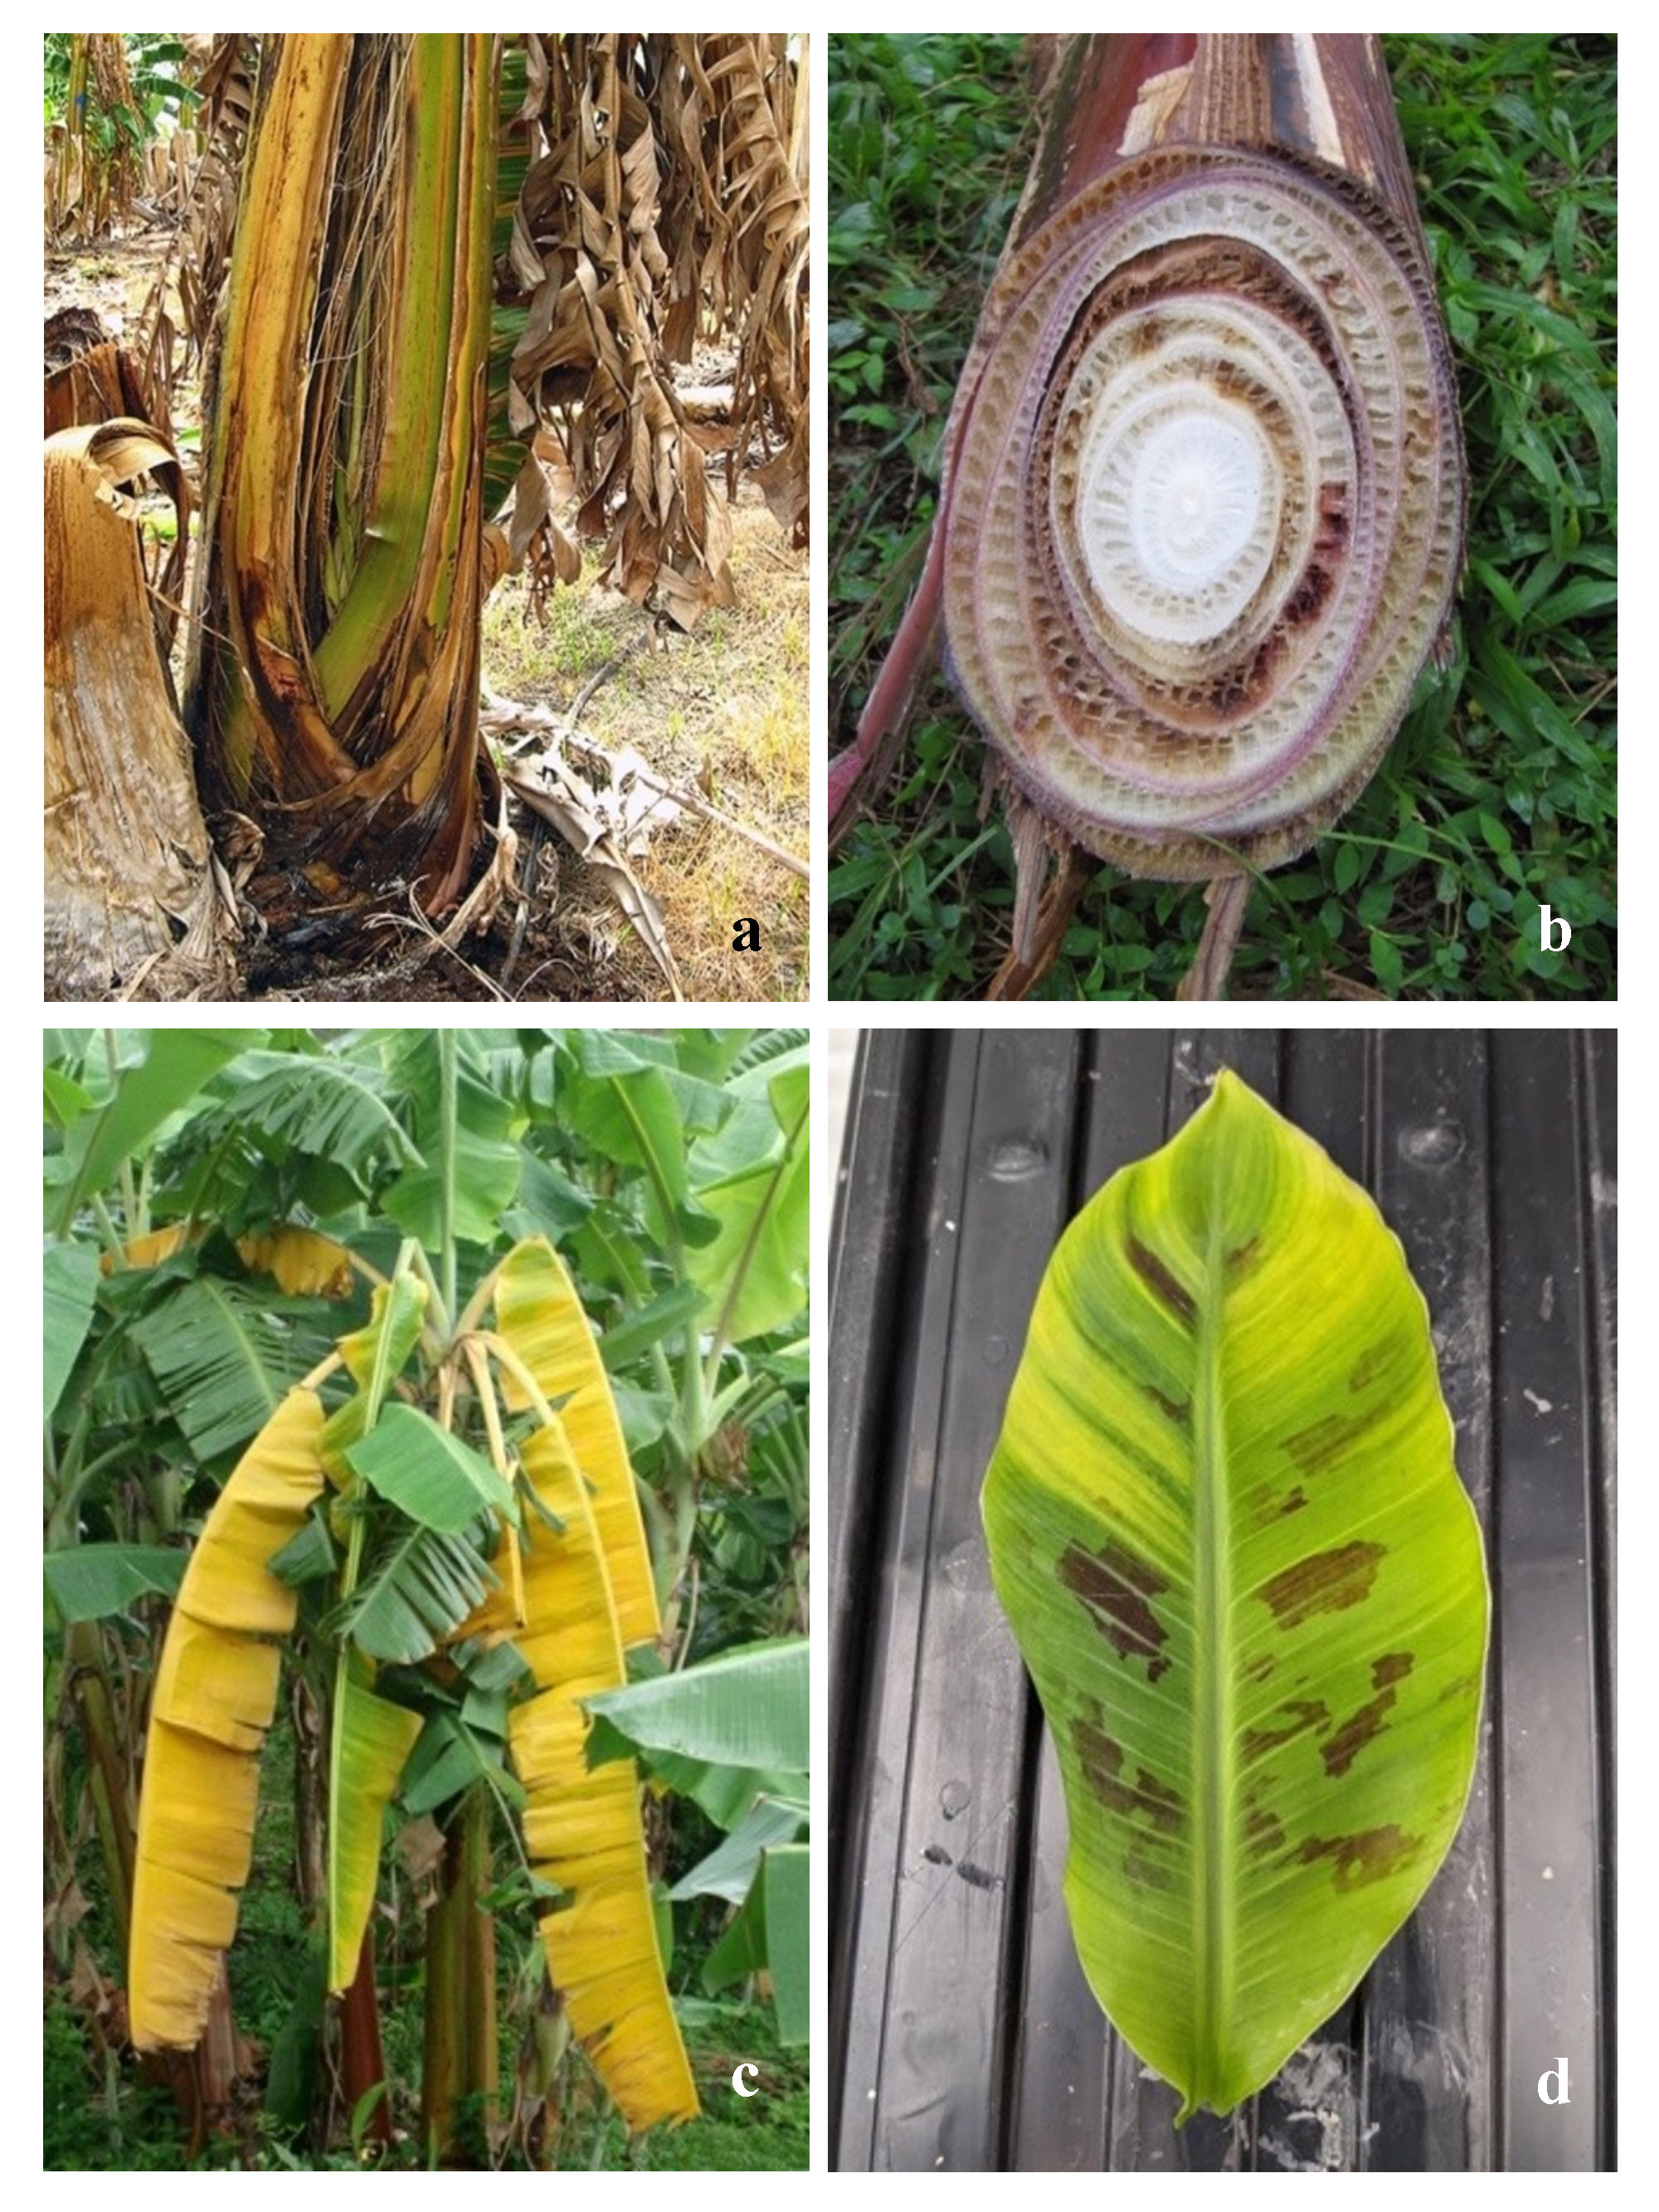
\includegraphics[width=15cm]{Figures/SymptomsofFoc.pdf}
    \caption[Typical symptoms of Fusarium  wilt of banana.]{\textbf{Typical symptoms of \textit{Fusarium} wilt of banana.} (a) Splitting of the psuedostem, (b) discolouration of the psuedostem, (c) yellowing of lower leaves, and (d), a streaking pattern is observed on the foliage.}
    \label{fig:FusariumWiltSymptoms}
\end{figure}

\subsection{Classification of \acl{Focub}}

\ac{Focub} belongs to the \ac{FOSC}. The species complex contains both plant and animal pathogens, as well as saprophytes and endophytes (Leslie and Summerell, 2006). \ac{Fo} has high functional and genetic diversity, shown plainly in its broad plant host range. The species complex can infect around 150 species of both monocotyledonous and dicotyledonous plants, including many horticulturally significant crops such as banana, tomato and lettuce  (Edel-Hermann and Lecomte, 2019).  Individual pathogenic \ac{Fo} isolates can infect only one or a few plant species. Plant pathogenic \ac{Fo} are therefore divided into ‘special forms’, or (\ac{fsp}), each of which is adapted to specific hosts (Snyder and Hansen, 1940). For instance, strains which cause Fusarium wilt in tomato are classified as \ac{Fol}. To date, 106 \ac{fsp} have been clearly described and with at least an additional 37 putative \ac{fsp} (Edel-Hermann and Lecomte, 2019).   

Some \ac{fsp} can be further subdivided into pathogenic races, determined by pathogenicity towards specific host cultivars. Three races of \ac{Focub} affecting banana have been identified. \acl{r1} affects banana cultivars such as ‘Gros Michel’ (AAA), ‘Maqueno’, ‘Silk’, ‘Pome’ (AAB), and ‘Pisang Awak’ (ABB); \acl{r2} affects ‘Bluggoe’ and other cooking bananas (ABB); Race 4 affects the subgroup Cavendish (AAA) as well as hosts of \ac{r1} and \ac{r2} (Ploetz, 2015a) and has been further divided into \ac{str4} (S\ac{tr4}) and  (\ac{tr4}). \ac{tr4} is distinguished from \ac{str4} as it affects susceptible cultivars without disease-predisposing conditions (Ploetz, 2015b).  

Identification of isolates based on race is often subjective. During the 1980s an additional method of \ac{Focub} identification based on \ac{vcg} was developed (Correll, 1991). \ac{vcg}s are comprised of isolates that possess the same alleles at all \ac{vic} loci, and so can form stable heterokaryons with each other (Correll, 1991). So far, 24 \ac{vcg}s of \ac{Focub} have been identified (Table ~\ref{tab:VCGTab}) (Czislowski \et 2018).  Some \ac{vcg}s of \ac{Focub} are taxonomically closer to other \ac{fsp} of \ac{Fo} than other \ac{Focub} \ac{vcg}s. This, coupled with distinct genetic lineages identified through phylogenetic analysis, has resulted in the recognition of a polyphyletic – taxonomic group including members from different ancestral lineages – evolutionary history for \ac{Focub} (Koenig \et 1997, Ploetz, 2006). 

Maryani \et (2019) recently revised the taxonomy of \ac{Focub}, generating the Fusarium of Banana Species Complex and proposing several new species. However, Torres-Bedoya \et (2021) have suggested that the revision is premature and that the data do not fully support the revision. There continues to be active debate surrounding \ac{Focub} classification and a clear, robust, universally accepted taxonomy has not yet been established. Race, although somewhat informal, remains the most widely accepted method of \ac{Focub} classification – whereby isolates are identified based on virulence towards specific host cultivars.  

%Insert the VCG table
% Please add the following required packages to your document preamble:
% \usepackage{longtable}
% Note: It may be necessary to compile the document several times to get a multi-page table to line up properly
\begingroup
\setlength{\tabcolsep}{28pt} % Default value: 6pt
\renewcommand{\arraystretch}{0.75}
\begin{longtable}[tc!]{ccc}
\caption[\acf{vcg} of \ac{Focub}]{{\textbf{\acf{vcg} of \ac{Focub}} and race (Czislowski \et 2018).} Cross-compatible VCGs can form VCG complexes.}
\label{tab:VCGTab}\\
\hline
\textbf{VCG} & \textbf{VCG   complex} & \textbf{Race}    \\ \hline
\endfirsthead
%
\multicolumn{3}{c}%
{{\bfseries Table \thetable\ continued from previous page}} \\
\endhead
%
0120  & 0120–01215           & STR4             \\
0121  &                      & R4               \\
0122  &                      & R4               \\
0123  &                      & R1               \\
0124  & 0124–0125–0128–01220 & R1,   R2         \\
0125  & 0124–0125–0128–01220 & R1, R2           \\
0126  &                      & R1               \\
0127  & No longer valid      & No longer valid  \\
0128  & 0124–0125–0128–01220 & R1,   R2         \\
0129  & 0129–01211           & STR4             \\
01210 &                      & R1               \\
01211 & 0129–01211           & STR4             \\
01212 &                      & Not   Identified \\
01213 & 01213–01216          & TR4              \\
01214 &                      & R2               \\
01215 & 0120–01215           & STR4             \\
01216 & 01213–01216          & TR4              \\
01217 &                      & R1               \\
01218 &                      & R1               \\
01219 &                      & Not identified   \\
01220 & 0124–0125–0128–01220 & R1               \\
01221 &                      & Not Identified   \\
01222 &                      & Not   Identified \\
01223 &                      & Not Identified   \\
01224 &                      & Not   Identified \\ \hline
\end{longtable}
\endgroup

\section{The \acl{Fo} genome} 

An emerging explanation for shared host specificity between different \ac{Fo} lineages relates to the compartmentalisation of the \acl{Fo} genome. A theory which has become increasingly prevalent in \acl{Fo} genomics since the publication of Comparative genomics reveals mobile pathogenicity chromosomes in Fusarium by Ma \et in 2010. The study explains that the \textit{Fusarium} genome can be organised into two parts containing either core chromosomes or accessory (lineage-specific/supernumerary) chromosomes and suggests that these accessory chromosomes can be horizontally transferred. A theory which has since been demonstrated in Fol (Vlaardingerbroek \et 2016a, Vlaardingerbroek \et 2016b, Li \et 2020a), \acl{Fo} f. sp. \textit{radicis-cucumerinum} (van Dam \et 2017) and \acl{Fo} f. sp. \textit{melonis} (Li \et 2020b). 

The 11 core chromosomes within the \acl{Fo} genome encode functions necessary for primary metabolism and reproduction (van Dam \et 2017).  The remaining accessory chromosomes, which vary in number among \ac{fsp}, are not required for primary metabolism and reproduction, contain secondary metabolite biosynthetic gene clusters, encode virulence genes such as effectors, and possess a high number of transposable elements (Ma \et 2010, Schmidt \et 2013, Witte \et 2021). The accessory chromosomes which are particularly important for virulence are referred to as pathogenicity chromosomes.  Pathogenicity chromosomes within \acl{Fo} are often characterised by the presence of effector genes (Ma \et 2010). Effectors are secreted proteins that play an essential role in fungal colonisation of plant hosts and plant immune responses (Lo Presti \et 2015).  

\subsection{Segmental Duplication Paper}

\subsection{The Plant Innate Immune System}

The plant’s innate immune system is comprised of two interconnect tiers which perceive and respond to pathogen infection (Han, 2019, Ngou \et 2022). The first tier recognises microbial- or \ac{pamp} which are slow-evolving, conserved molecules (such as the fungal cell wall component, chitin) using transmembrane \ac{prr} on the plant cell surface. Once \ac{pamp} have been recognised, \ac{pti} is induced (Jones and Dangl, 2006). \ac{pti} responses include numerous cell signalling events such as altered ion fluxes, the production of apoplastic reactive oxygen species, callose deposition, and transcriptional reprogramming (Figure:~\ref{fig:PlantImmuneSystem}) (Han, 2019, DeFalco and Zipfel, 2021). 

\begin{figure}[h!]
    \centering
    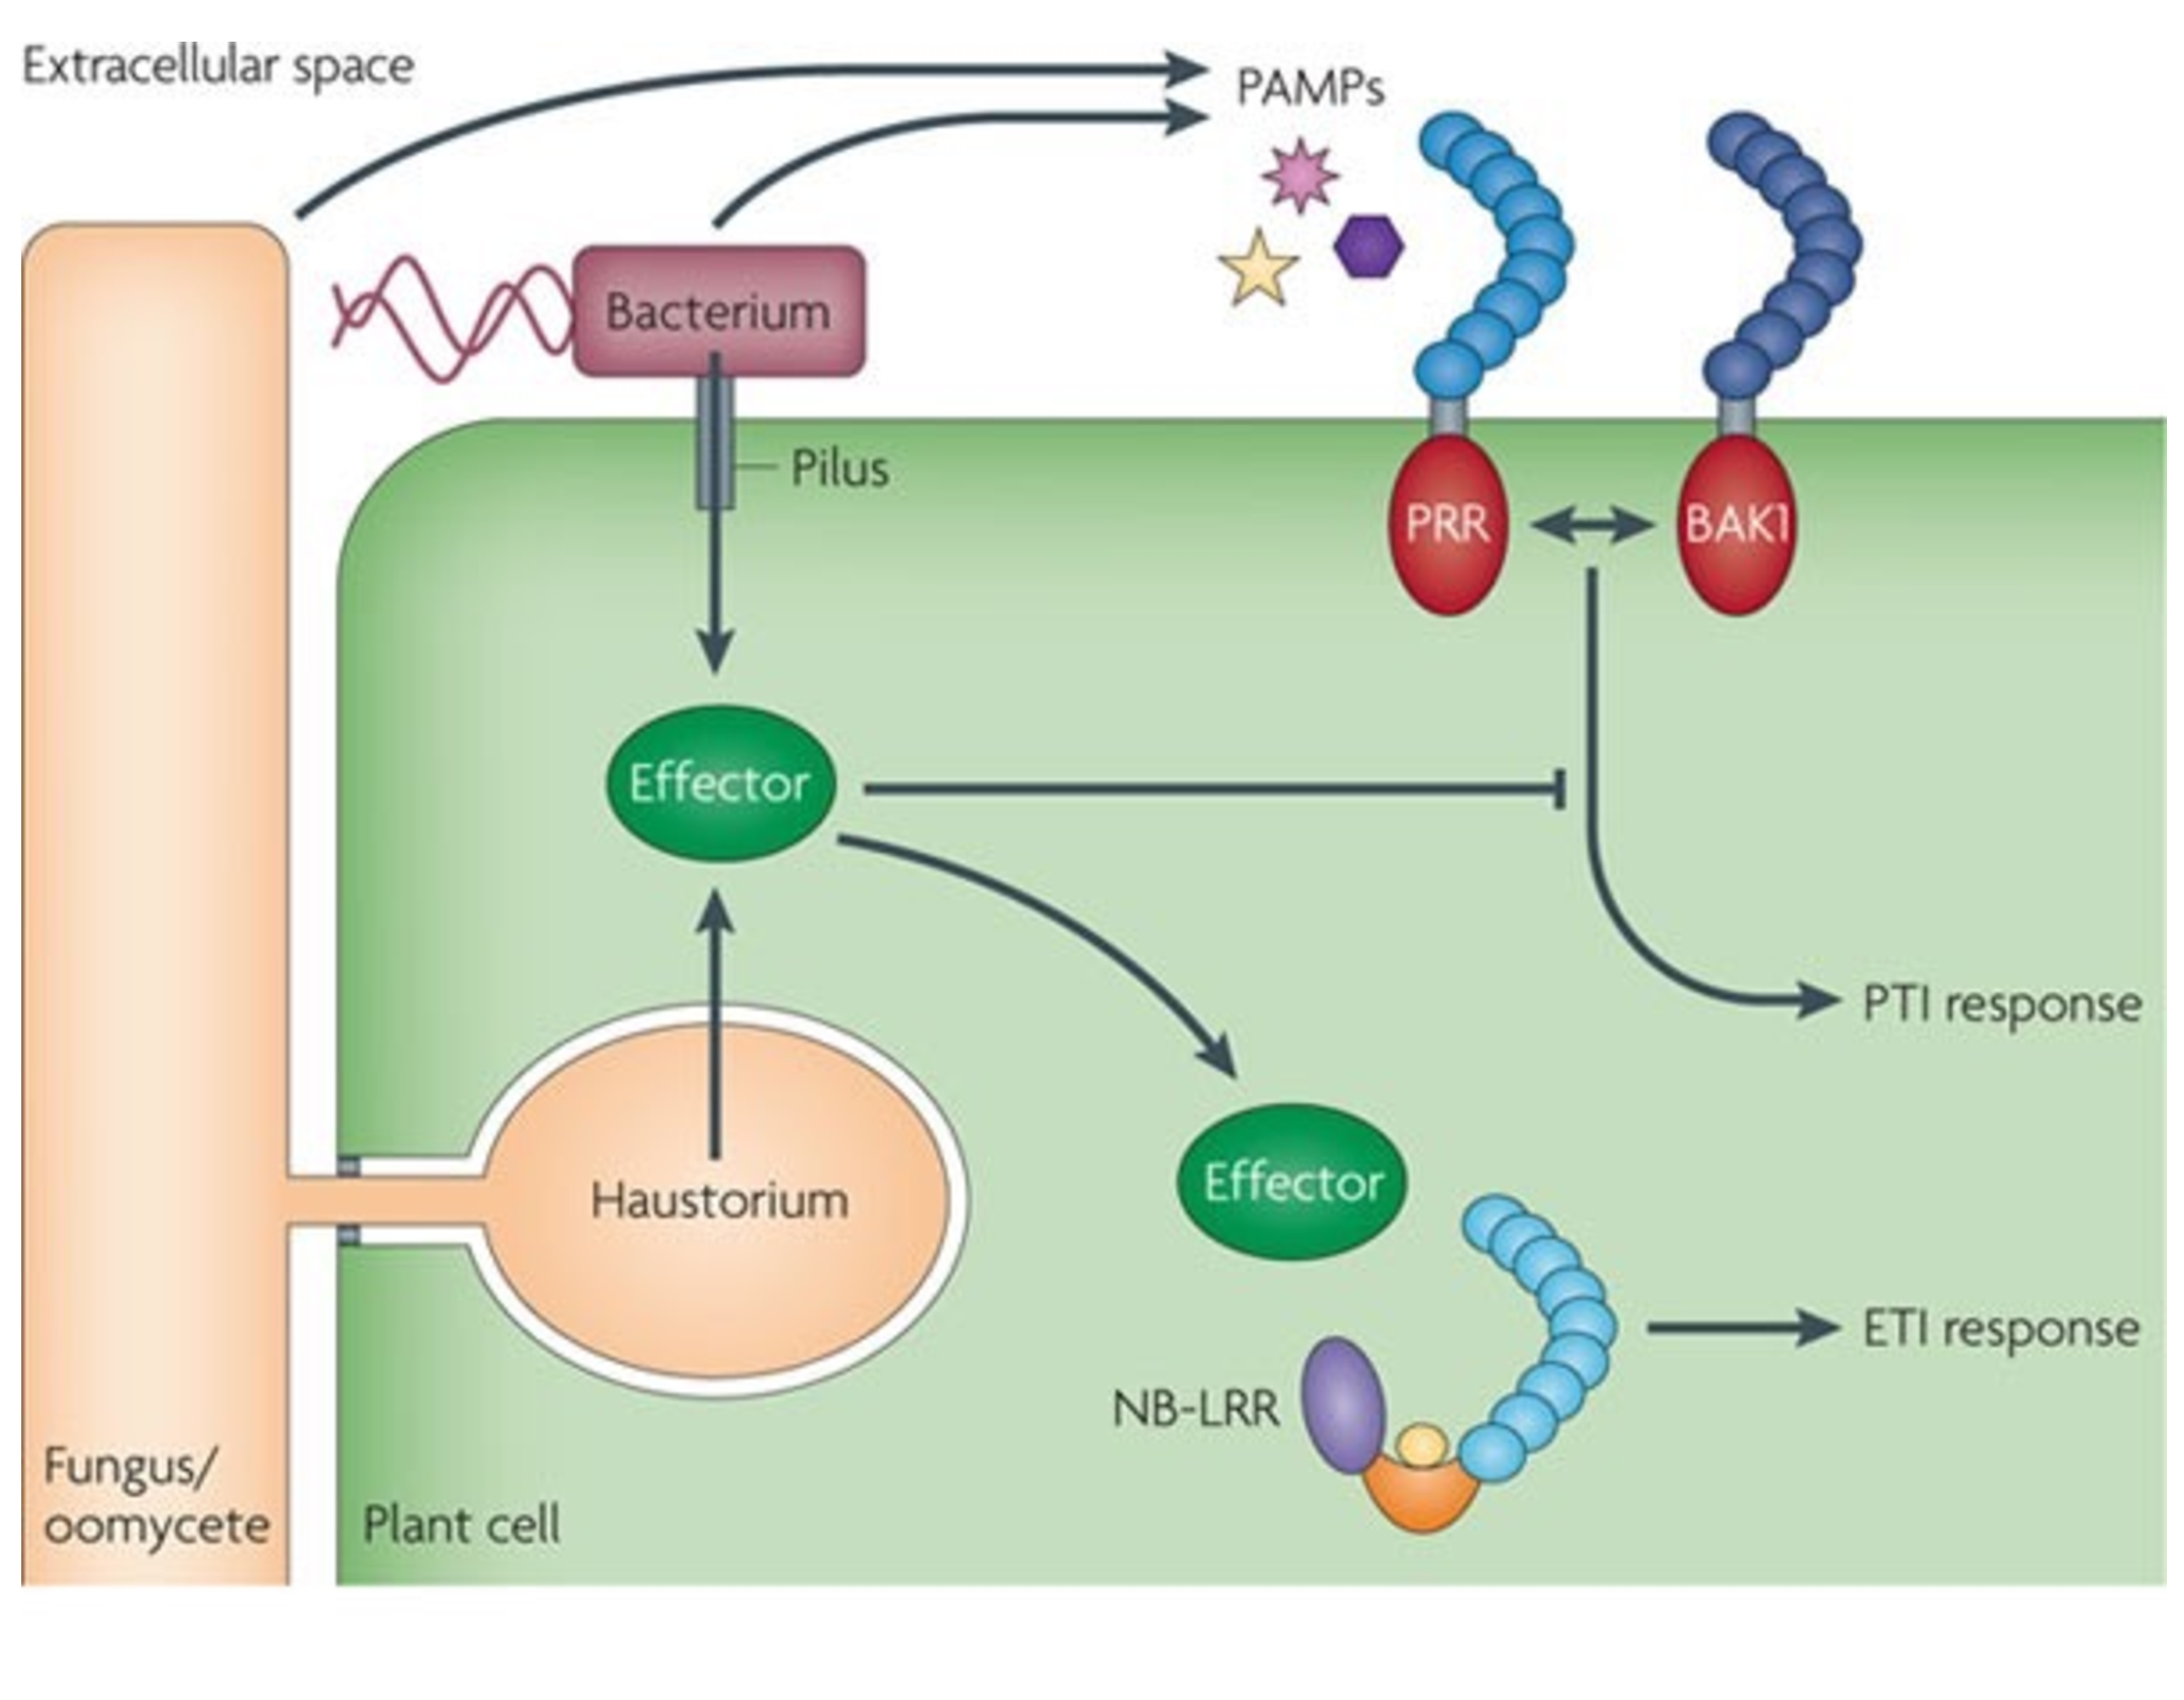
\includegraphics[width=14cm]{Figures/DoddsArticleModel.pdf}
    \caption[Overview of the plant immune system.]{\textbf{Overview of the plant immune system.} Pattern recognition receptors (PRRs) perceive microbial- pathogen-associated molecular patterns (MAMPs/PAMPs) and induce a PAMP-triggered immunity (PTI) response from the host. In order to overcome host cell defences, pathogens secrete small molecules known as effectors into the host cell, inducing effector-triggered susceptibility (ETS). Plants have adapted a family of resistance proteins (R proteins), which can perceive pathogen effectors (avirulence proteins) and stimulate an effector-triggered immunity (ETI) response from the plant host (From Dodds and Rathjen, 2010).}
    \label{fig:PlantImmuneSystem}
\end{figure}

To evade, suppress or interfere with \ac{pti} responses and establish infection, fungal pathogens secrete proteins termed ‘effectors’ into the host cell which results in \ac{{ets} (Jones and Dangl, 2006, Ngou \et 2022). To combat \ac{ets}, plants possess a suite of \ac{rprot} which perceive effectors (termed ‘\ac{avr} effectors’) and induce further immune responses termed \ac{eti} (Jones and Dangl, 2006). \ac{rprot} are conserved intracellular receptors of the \ac{nlr} class. The structure, function, and effector perception (direct or indirect) of \ac{rprot} is variable and often specific (see: Chen \et 2022, Wang \et 2022). Similarly, effectors are typically highly variable and specific to individual pathogens (Lo Presti \et 2015).  


\subsection{The \acl{Fo} Effectorome}

In the \ac{FOSC}, the only family of effectors so far identified are the \ac{sixg}. In total, 14 SIX proteins (SIX1 – SIX14) have been identified through mass spectrometry of infected tomato xylem sap and whole genome sequencing (Houterman \et 2007, Schmidt \et 2013).  All 14 \ac{sixg}s are found on the pathogenicity chromosome in \ac{Fol} (Ma \et 2010, Schmidt \et 2013), and studies have confirmed that \textit{SIX1, SIX2, SIX3, SIX5} and \textit{SIX6} are essential for conferring virulence in tomato, with  \textit{SIX4} (\textit{Avr1}), \textit{SIX3} (\textit{Avr2}) and \textit{SIX1} (\textit{Avr3}) all recognised by corresponding \ac{rprot} (called ‘I’ for Immunity) in tomato (Rep \et 2004, Houterman \et 2007, Lievens \et 2009, Takken and Rep, 2010, Gawehns \et 2014, Ma \et 2015).  

Since their discovery in \ac{Fol}, homologs of \ac{sixg}s have been identified in other \ac{fsp}, including \textit{cepae, conglutinans, fragariae, melonis, pisi, radicis-cucumerinum,} and \textit{vasinfectum} (Czislowski \et 2018). A further \textit{SIX} gene, (\textit{SIX15}) has been described by Simbaqueba \et (2018) in \acl{Fo} f. sp. \textit{physalis}, although \textit{SIX15} is not widely reported.  

In \ac{Focub}, homologs of \textit{SIX1, SIX2, SIX4, SIX6, SIX7, SIX8, SIX9}, and \textit{SIX13} have been identified (Czislowski \et 2018, An \et 2019), and \textit{SIX1} and \textit{SIX8} have been recognised in \ac{Focub} \ac{tr4} as essential for virulence through knockout mutants (Widinugraheni \et 2018, An \et 2019). Czislowski \et (2018) reported differences in the \ac{sixg} repertoire of \ac{Focub} \ac{r1} and R4 lineages and hypothesised that the differences in \ac{sixg} profiles contribute to the variability in the \ac{Focub} host cultivar range.  However, as the authors point out, \ac{sixg}s are unlikely to be the only set of effectors involved in host specificity, and state ‘it should be expected that novel and undiscovered effectors remain to be identified in the lineages of \ac{Focub}’ (Czislowski \et 2018 pp. 1168).  

Ma \et (2010) showed that the pathogenicity chromosomes in \ac{Fol}, have a high number of retro-elements, including the non-autonomous class II \ac{te}, \ac{mites}. A specific family of \ac{mites}, known as \ac{mimp}s, are found upstream of all known \ac{sixg} in \ac{Fol} (Schmidt \et 2013). Characterised by their \ac{tir} sequence and short length (180–220 \ac{bp}), Schmidt \et (2013) surmised that \textit{mimps} could be used for the prediction of effectors in \acl{Fo}, particularly \ac{sixg}s, a theory which was later demonstrated by van Dam \et (2016), van Dam and Rep, (2017) and (Armitage \et 2018). 

The hypothesis that effector profiles contribute to host specificity is reported for other \ac{fsp} (Achari \et 2021, Batson \et 2021) and is argued on the host species level for the \ac{FOSC} (van Dam \et 2016). With advances in genome sequencing and analysis, it is possible to identify new candidate effectors using common characteristics shared between known effectors in \ac{Fol}, in other \ac{fsp}.

\section{Control of \acl{Focub}}

There are few effective controls for \ac{Focub} in the wider environment. Chlamydospores can persist in the soil for decades and \ac{Focub} can invade non-host plants and survive as an endophyte, with grass and weed species acting as sources of inoculum (Pegg \et 2019). Biological control agents and fungicides have been investigated as a means of \ac{Focub} control. However, most of these are \textit{in vitro} and greenhouse assays which, although successful, are not practical or effective in-field. (Moses, 2016, Chan \et 2017, Dita \et 2018).  

As most commercial bananas are triploid and parthenocarpic conventional breeding for resistance is exceedingly challenging (Dale \et 2017b). One somaclonal variant of Cavendish, ‘Formosana’ is marketed as being resistant to \ac{tr4}, however, yields are slightly reduced due to its longer growth cycle and there have been reports of  ‘Formosana’ showing \ac{tr4} susceptibility in later field trials (Lee \et 2011, Dale \et 2017a). A further somaclonal variant, ‘Guijiao 9’, is also marketed as showing lower disease severity compared to conventional commercial Cavendish varieties such as ‘Williams’ (Sun \et 2019), but, the variety has only recently been released to the market and field trials outside of the region in which this variety was developed have not yet been conducted.  

Advances in genetic modification technologies have facilitated the development of two \ac{tr4}-resistant transgenic Cavendish lines (Dale \et 2017). One of these lines, ‘QCAV-4’ is currently undergoing regulatory approval in Australia (Lu, 2023). The transgenic 'QCAV-4' variety was generated by transforming \textit{M. acuminata }Cavendish cv. 'Grand Naine' (AAA subgroup) embryogenic cell suspensions (prepared from immature male flowers) using the centrifugation assisted \textit{Agrobacterium tumefaciens}-mediated method with \ac{rga2}.\ac{rga2} is a putative \ac{nlr}-type \ac{rgene} from a seedling of \textit{Musa acuminata} ssp. \textit{malaccensis} with resistance to \ac{Focub4}. However, the market for genetically modified crops within Europe is limited, although debate and legislation are currently under review and development. 

Gene-edited banana may be a more marketable alternative, particularly for Europe, and editing for disease resistance has been demonstrated in banana. Tripathi \et (2021) used CRISPR-Cas9 to make mutations to the downy mildew resistance 6 (DMR6) orthologue in banana, showing enhanced resistance to the bacterial pathogen \ac{xvm}, this approach may be applied to target a gene which could provide resistance to \ac{Focub}.  

\subsection{The Role of Diagnostics in Banana Disease Detection and Management}

Prevention of \ac{Focub} introduction has so far proven the most effective method of \ac{Focub} control on a large scale (Ploetz, 2015b), with management primarily focused on hygiene practices. Therefore, emphasis has been placed on the development of accessible, fast, and accurate diagnostic tools (Ordóñez \et 2019). Molecular and image-based diagnostics have both been developed to identify \ac{Focub}. However, many of the current image-based diagnostics are currently unable to distinguish Foc from other banana wilt pathogens, and the molecular assays struggle to accurately identify pathogenic races.  
 

\section{Advancements in tech for diagnosing plant diseases}
\subsection{genomics?}
\subsection{imaging?}
\subsection{metabolomics? Human diseases?}


\newpage
\section{Project Aims and Objectives}

The overall aim of this research is to develop tools for the detection of \acl{Focub} \ac{tr4} in banana and contribute towards understanding of \acl{Focub} classification, identification, and infection and banana responses. 

\begin{enumerate}
    \item Build tools which aid in the identification of targets for molecular diagnostics and contribute to our understanding of \ac{Focub}-banana interactions as well as the evolutionary history and classification of \ac{Focub}. 
    \item Develop molecular diagnostics which can be used to identify specific races of \acl{Fo}. \footnote{Due to challenges sourcing isolates and sequence information from collaborators in Tamil Nadu Agricultural University, India (TNAU), our effector identification tool cannot currently be validated using Foc. However, we are testing this tool using other \acl{Fo} \ac{fsp} with collaborators at NIAB and the University of Warwick.}
    \item Employ phenomics to investigate banana responses to \ac{Focub} infection and contribute to the development of image-based diagnostic techniques.  
    \item Develop novel -omics approaches to improve understanding of banana interactions with \ac{Focub}.  
\end{enumerate}

\newpage
\section{Thesis Structure}

\subsection{Chapter 2: Potential Novel \textit{Fusarium} Pathogen of Banana Identified} 

This chapter will review the comparative genome assembly and subsequent analysis performed on \textit{Fusarium} isolates collected by collaborators at Tamil Nadu Agricultural University in India. Phylogeny of isolates and geographic distribution will be discussed compared to publicly available genomes, and a potential novel species presented. 

\subsection{Chapter 3: Improving Genomic Tools for Identifying Virulence Factors in \textit{Fusarium oxysporum}} 

This chapter will chart the development of the \textit{Mimp} Associated Effector Identification (Maei) tool which identifies effectors in \acl{Fo}, and the implications effector profiles have on the classification and genome compartmentalisation of the FOSC. It will include new genome sequences from collaborators at UoW and NIAB. Effector presence, location, predicted structures, homology, expression, and potential function will be explored. 
These candidate effectors will be used in the development of molecular diagnostics, and the potential of the Maei tool in the development of \acl{Fo} \ac{fsp} race-specific diagnostics will be explored. 

\subsection{Chapter 4: Phenomics: Image-based Analysis of Banana Stresses}

Banana disease imaging will be conducted and discussed, exploring the technologies currently available for image-based disease detection in banana, how spectral data can distinguish stresses, and why different spectral patterns are observed. 
We will also explore CT and microscopy data, recording the internal development of symptoms and how this relates to multispectral data. This data will also be discussed in chapter 4. 

\subsection{Chapter 5: Metabolomics: The Banana-pathogen Metabolome}
Untargeted Metabolomics analysis will be performed on infected banana to help develop our understanding of the \acl{Focub} infection process and indicate how this may be related to patterns observed in image-based analysis. We also identify specific markers of infection from a variety of biotic and abiotic stresses. 

\subsection{Chapter 6: General Discussion}
This chapter will discuss the main results from the thesis and will draw overall conclusions. It will also consider areas for improvement and future work. 


 

 



 



 



 